\addchap{A Anmerkung zur Nutzung von Künstlicher Intelligenz}
\setcounter{chapter}{1}

Im Rahmen dieser Arbeit wurden Künstliche Intelligenz (\acrshort{acr:KI})\index{Künstliche Intelligenz} basierte Werkzeuge benutzt. Tabelle~\ref{tab:anhang_uebersicht_KI_werkzeuge} gibt eine Übersicht über die verwendeten Werkzeuge und den jeweiligen Einsatzzweck.

\begin{table}[hbt]	
	\centering
	\renewcommand{\arraystretch}{1.5}	% Skaliert die Zeilenhöhe der Tabelle
	\captionabove[Liste der verwendeten Künstliche Intelligenz basierten Werkzeuge]{Liste der verwendeten \acrshort{acr:KI}-basierten Werkzeuge}
	\label{tab:anhang_uebersicht_KI_werkzeuge}
	\begin{tabular}{>{\raggedright\arraybackslash}p{0.3\linewidth} >{\raggedright\arraybackslash}p{0.65\linewidth}}
	\textbf{Werkzeug} & \textbf{Beschreibung der Nutzung}\\
	\hline 
	\hline
	Microsoft Copilot &
	\vspace{-\topsep}
	\begin{itemize}[noitemsep,topsep=0pt,partopsep=0pt,parsep=0pt] 
		\item Unterstützung bei der Programmierung (z. B. Code-Vorschläge und Strukturierung)
		\item Hilfe bei der sprachlichen Formulierung und Verbesserung von Satzstrukturen (gesamt)
		\item Zusammenfassung und Aufbereitung von wissenschaftlichen Texten als Grundlage für eigene Formulierungen (gesamt)
	\end{itemize} \\ 
	
	DeepL & 
	\vspace{-7.5mm}
	\begin{itemize}
		\item Verbesserung von Satzstrukturen und Formulierungen (gesamt)
	\end{itemize}\\
	\hline 
\end{tabular}
\end{table}

\addchap{B Ergänzungen}
\setcounter{chapter}{2}


\section{Details, welche im Hauptteil den Lesefluss behindern}


\begin{figure}[htbp]
    \centering
    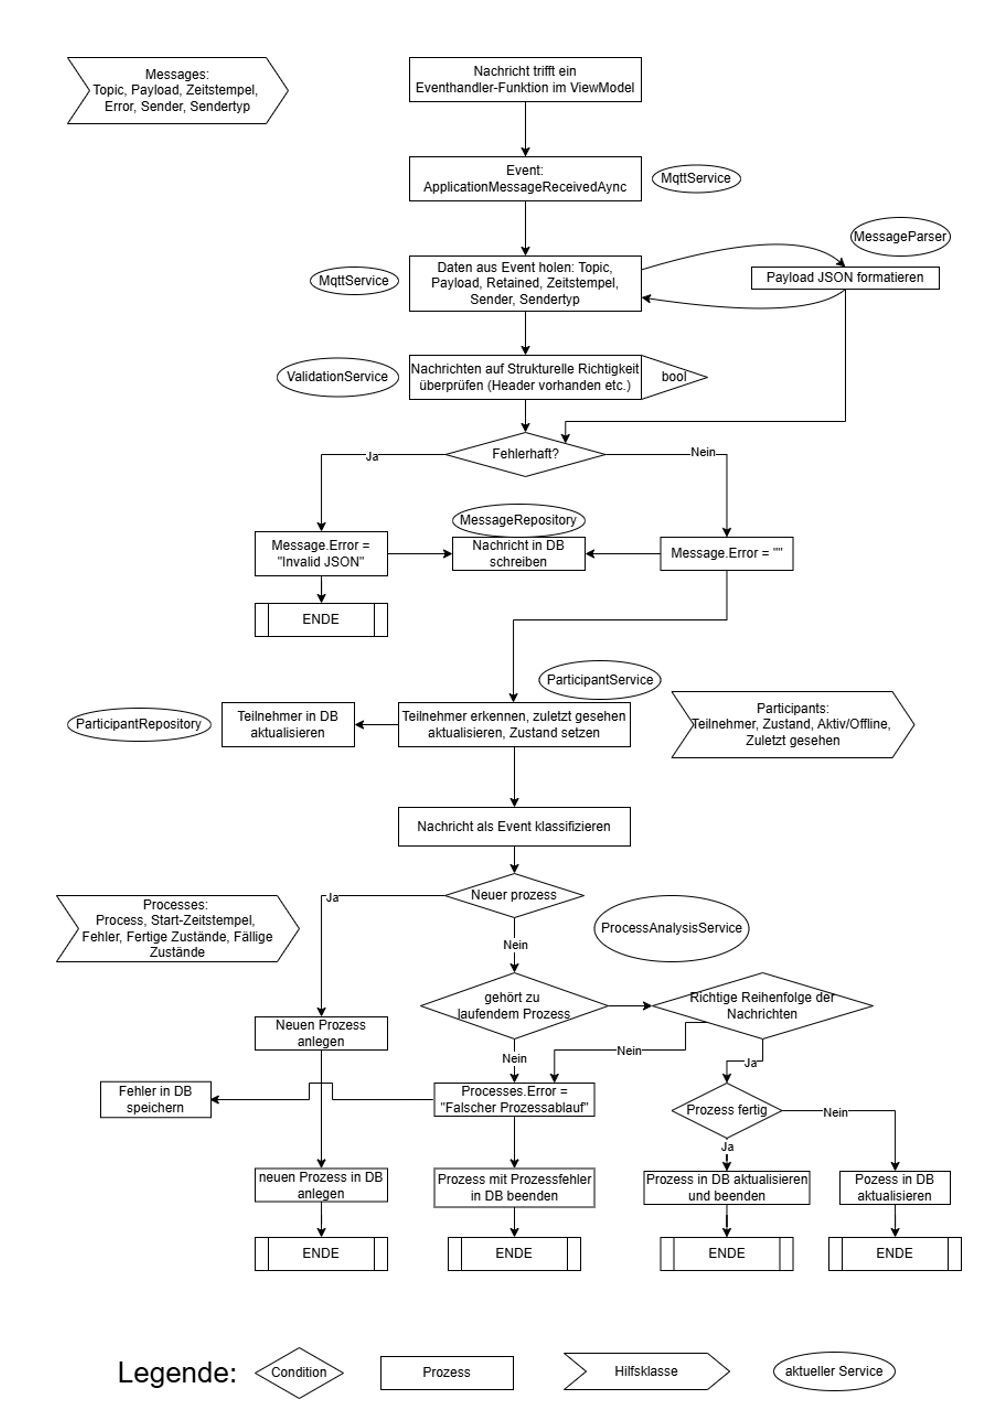
\includegraphics[width=0.8\textwidth]{images/floatchartmessages.png}
    \caption{Floatchart-Diagramm für die Nachrichtenverarbeitung}
    \label{fig:FloatchartMessages}
\end{figure}

\begin{longtable}{p{2.5cm} p{12cm}}
    \caption{Übersicht der Automatisierungsabläufe} 
    \label{tab:automatisierungsabläufe} \\ 
    \toprule \textbf{Prozess} & \textbf{Beschreibung} \\ 
    \midrule \endfirsthead \toprule \textbf{Prozess} & \textbf{Beschreibung} \\ 
    \midrule \endhead Linienstopp & \begin{itemize} \item Anfangstopic \begin{itemize} \item mlc/v1/cmd/desired/\{MLC\} \item messageType: T\_EXTERNAL\_LINE\_COMMAND\_\-DESIRED\_EVENT \item commandString: LINE\_STOP \end{itemize} \item Erwartete Topics \begin{itemize} \item mlc/v1/omac/reported/\{machineName\} \end{itemize} \item Zusatzinformationen \begin{itemize} \item Durchlaufene OMAC-Zustände: STOPPING, STOPPED \end{itemize} \end{itemize} \\ 
    \midrule Linienstart & \begin{itemize} \item Anfangstopic \begin{itemize} \item mlc/v1/cmd/desired/\{MLC\} \item messageType: T\_EXTERNAL\_LINE\_COMMAND\_\-DESIRED\_EVENT \item commandString: LINE\_START \end{itemize} \item Erwartete Topics \begin{itemize} \item mlc/v1/omac/reported/\{machineName\} \end{itemize} \item Zusatzinformationen \begin{itemize} \item Durchlaufene OMAC-Zustände: RESETTING, IDLE, STARTING, EXECUTE \end{itemize} \end{itemize} \\ 
    \midrule Linienquittierung & \begin{itemize} \item Anfangstopic \begin{itemize} \item mlc/v1/cmd/desired/\{MLC\} \item messageType: T\_EXTERNAL\_LINE\_COMMAND\_\-DESIRED\_EVENT \item commandString: LINE\_QUIT \end{itemize} \item Erwartete Topics \begin{itemize} \item mlc/v1/cmd/desired/\{MLC\} (Bestätigung der MLC) \item diagnosis/v1/messagesAcknowledged/reported/\{ma\-chineName\} \end{itemize} \item Zusatzinformationen \begin{itemize} \item Alle Maschinen mit Fehler müssen die Fehlernachrichtquittierung bestätigen. \end{itemize} \end{itemize} \\ 
    \midrule Artikelwechsel & \begin{itemize} \item Anfangstopic \begin{itemize} \item mlc/v1/conf/desired/\{MLC\} \item Linienartikel \item Teilnehmer am Artikelwechsel \end{itemize} \item Erwartete Topics \begin{itemize} \item mlc/v1/lineArticle/reported/\{machineName\} \end{itemize} \item Zusatzinformationen \begin{itemize} \item Maschinenartikel, der von den jeweiligen Teilnehmern geladen werden musste. \end{itemize} \end{itemize} \\ 
    \midrule Leerfahren & \begin{itemize} \item Anfangstopic \begin{itemize} \item mlc/v1/conf/desired/{MLC} \item desiredAction: RunEmpty \item Teilnehmer am Leerfahren \end{itemize} \item Erwartete Topics \begin{itemize} \item mlc/v1/batch/reported/\{machineName\} \end{itemize} \end{itemize} \\ \midrule Fliegender Artikelwechsel & \begin{itemize} \item Anfangstopic \begin{itemize} \item mlc/v1/continuousArticleChange/parameterSets/hand\-over/\{machineName\}/reported/\{MLC\} \end{itemize} \item Erwartete Topics \begin{itemize} \item mlc/v1/continuousArticleChange/parameterSets/hand\-over/reported/\{machineName\} \item mlc/v1/articleChange/producingBatches/reported/\{MLC\} \end{itemize} \end{itemize} \\ 
    \bottomrule 
\end{longtable}

 \begin{longtable}{|p{1cm}|p{3cm}|p{4.0cm}|p{4.8cm}|p{2cm}|} \caption{Ergebnisse der durchgeführten Funktionstests} \label{tab:funktionstests} \\
    \hline \textbf{Test-ID} & \textbf{Testfall} & \textbf{Testdurchführung} & \textbf{Erwartetes Ergebnis} & \textbf{Ergebnis} \\ \hline FT-01 & Verbindungsuf\-bau & Verbindung mit gültigem Broker herstellen & Verbindung wird aufgebaut und angezeigt & X 
    \\ \hline FT-02 & Ungültige Broker-IP & Falsche IP-Adresse eintragen & 5 Sekunden lang versuchen, dann Fehlermeldung anzeigen & X 
    \\ \hline FT-03 & Ungültiger Broker-Port & Falschen Port eintragen & 5 Sekunden lang versuchen, dann Fehlermeldung anzeigen & X 
    \\ \hline FT-04 & Manuelle Verbindungstrennung & Brokerverbindung manuell trennen & Verbindung wird getrennt und angezeigt & X 
    \\ \hline FT-05 & Verbindungs-Abbruch & Netzwerkkabel wird entfernt & Verbindungsabbruch wird in unter 3 Sekunden erkannt und Fehlermeldung wird angezeigt & X 
    \\ \hline FT-06 & Nachrichten\-empfang & Maschine sendet kontinuierlich Nachrichten; empfangene Nachrichten werden mit MQTT.fx verglichen & Alle Nachrichten werden empfangen & X 
    \\ \hline FT-07 & Pagination & Nachrichtenliste mit mindestens 3000 Nachrichten wird ganz durchgeblättert & Alle Nachrichten werden korrekt nachgeladen und gelöscht & X 
    \\ \hline FT-08 & Topic-Filterung & Verschiedene Topic-Filter wählen & Alle passenden Nachrichten werden gefunden und angezeigt & X 
    \\ \hline FT-09 & Suchfunktion & Verschiedene Teilnehmernamen, Uhrzeiten und Nachrichten werden eingegeben & Alle passenden Nachrichten werden gefunden und angezeigt & X 
    \\ \hline FT-10 & Datenbank-Speicherung & Nachrichten empfangen und Anwendung erneut laden & Gespeicherte Nachrichten bleiben erhalten & X 
    \\ \hline FT-11 & Teilnehmer-Erkennung & Retain-Nachrichten empfangen & Alle Teilnehmer ohne ,,integrated By'' richtig anzeigen & X 
    \\ \hline FT-12 & Zustands- und Statuserfassung & Alle OMAC-States von jedem Teilnehmer senden und empfangen & Zustände werden korrekt gespeichert und angezeigt & X 
    \\ \hline FT-13 & Regulärer Prozessablauf & Verpackungslinie durchläuft Prozess und beendet ihn korrekt & Prozess wird erkannt und ohne Fehler abgespeichert & -- 
    \\ \hline FT-14 & Fehlerhafter Prozess & Maschine durchläuft Prozess, beendet diesen jedoch nicht & Prozess wird erkannt und mit Fehler abgespeichert & X 
    \\ \hline FT-15 & Prozessfehler erkennen & Maschine durchläuft Prozess, beendet diesen jedoch nicht & Prozessfehler wird erkannt und in den Fehlermeldungen angezeigt & X 
    \\ \hline FT-16 & Strukturfehler erkennen & Alle verschiedenen Strukturfehler senden & Alle Strukturfehler werden richtig erkannt, angezeigt und können angeklickt werden & X 
    \\ \hline FT-17 & Linienfehler anzeigen & Maschine sendet drei verschiedene linieninterne Fehlermeldungen & Fehler und Sender werden erkannt, angezeigt und sind anklickbar & X \\ \hline  
\end{longtable}

\addchap{C Zusatzinformationen zu verwendeter Software}
\setcounter{chapter}{3}
\setcounter{section}{0}
\setcounter{table}{0}
\setcounter{figure}{0}

\section{Elektronischer Anhang}
Der vollständige Quellcode der im Rahmen dieser Arbeit entwickelten Anwendung wird aufgrund seines Umfangs nicht vollständig in der Arbeit dargestellt. Der Quellcode ist im folgenden Repository verfügbar: \url{https://github.com/Fabse6/MQTTAnalyzer}
\section{Wichtige Teile des Quellcodes}
\begin{lstlisting}[
    language={[Sharp]C},
    caption={MQTTMonitor: Programmcode für Verarbeitung und Darstellung empfangener MQTT-Nachrichten},
    label={lst:inflightpage}
    ]
public InflightPageViewModel(MqttClientService mqttClientService)
{
    _mqttClientService = mqttClientService;
    // Registrierung auf eingehende MQTT-Nachrichten
    _mqttClientService.ApplicationMessageReceived += OnApplicationMessageReceived;
    // Reaktiver Filter basierend auf Benutzereingabe
    var filter = this.WhenAnyValue(x => x.FilterText)
        .Throttle(TimeSpan.FromMilliseconds(800))
        .Select(BuildFilter);
    // Datenpipeline: Quelle -> Filter -> UI-Bindung
    _itemsSource.Connect()
        .Filter(filter)
        .ObserveOn(RxApp.MainThreadScheduler)
        .Bind(out _items)
        .Subscribe();
}
// Verarbeitung eingehender Nachrichten
Task OnApplicationMessageReceived(MqttApplicationMessageReceivedEventArgs eventArgs)
{
    return AppendMessage(eventArgs.ApplicationMessage);
}
// Hinzufügen neuer Nachrichten zur Datenquelle
public Task AppendMessage(MqttApplicationMessage message)
{
    return Dispatcher.UIThread.InvokeAsync(() =>
    {
        var newItem = CreateItemViewModel(message);
        _itemsSource.Add(newItem);
    }).GetTask();
}
// Erstellung des Filters
Func<InflightPageItemViewModel, bool> BuildFilter(string? searchText)
{
    if (string.IsNullOrEmpty(searchText))
    {
        return t => true;
    }
    return t => t.Topic.Contains(searchText, StringComparison.OrdinalIgnoreCase);
}
\end{lstlisting}

\begin{lstlisting}[
language=Python,
caption={Aufzeichnung von CPU-Auslastung und Arbeitsspeicherverbrauch},
label={lst:pythontaskmanager}
]
import time
import csv
import sys
import psutil

TARGET_PROCESS = "MQTTAnalyzer.exe"
INTERVAL_SECONDS = 0.1  # 100 ms
CSV_FILENAME = "mqtt_analyzer_log.csv"
MATLAB_SCRIPT = "plot_mqtt_data.m"


def find_process(process_name):
    for proc in psutil.process_iter(['pid', 'name']):
        try:
            if proc.info['name'] and proc.info['name'].lower() == process_name.lower():
                return proc
        except (psutil.NoSuchProcess,
                psutil.AccessDenied,
                psutil.ZombieProcess):
            pass

    return None



def main():
    print(f"Suche nach Prozess {TARGET_PROCESS} ...")

    proc = find_process(TARGET_PROCESS)

    if proc is None:
        print(f"Fehler: Prozess '{TARGET_PROCESS}' wurde nicht gefunden.")
        sys.exit(1)

    print(f"Prozess gefunden! (PID: {proc.pid})")
    print(f"Messung alle {INTERVAL_SECONDS} Sekunden")
    print("Beenden mit Strg+C\n")

    proc.cpu_percent()
    time.sleep(INTERVAL_SECONDS)

    max_cpu = 0.0
    max_ram_mb = 0.0
    total_cpu = 0.0
    total_ram = 0.0
    count = 0

    start_time = time.time()

    with open(CSV_FILENAME, "w", newline="", encoding="utf-8") as file:
        writer = csv.writer(file)

        writer.writerow([
            "Zeitstempel",
            "Zeit_Sekunden",
            "CPU_Prozent",
            "RAM_MB"
        ])

        try:
            while True:
                if not proc.is_running():
                    print("\nProzess wurde beendet.")
                    break

                elapsed = time.time() - start_time

                timestamp = (
                    time.strftime("%Y-%m-%d %H:%M:%S")
                    + f".{int((elapsed % 1) * 1000):03d}"
                )

                cpu = proc.cpu_percent(interval=None)
                ram_mb = proc.memory_info().wset / (1024 * 1024)

                max_cpu = max(max_cpu, cpu)
                max_ram_mb = max(max_ram_mb, ram_mb)

                total_cpu += cpu
                total_ram += ram_mb
                count += 1

                writer.writerow([
                    timestamp,
                    f"{elapsed:.3f}",
                    f"{cpu:.2f}",
                    f"{ram_mb:.2f}"
                ])

                file.flush()

                time.sleep(INTERVAL_SECONDS)

        except KeyboardInterrupt:
            print("\nAufzeichnung manuell beendet.")

    if count > 0:
        avg_cpu = total_cpu / count
        avg_ram = total_ram / count

        print("\n" + "=" * 50)
        print(f"Zusammenfassung ({count} Messungen)")
        print("=" * 50)
        print(f"Max CPU-Auslastung:               {max_cpu:.2f} %")
        print(f"Durchschnittliche CPU-Auslastung: {avg_cpu:.2f} %")
        print(f"Maximaler RAM-Verbrauch:          {max_ram_mb:.2f} MB")
        print(f"Durchschnittlicher RAM-Verbrauch: {avg_ram:.2f} MB")

    print(f"\nMATLAB-Skript erstellt: {MATLAB_SCRIPT}")
    print(f"CSV-Datei erstellt:     {CSV_FILENAME}")


if __name__ == "__main__":
    main()
\end{lstlisting}

\clearpage
